\documentclass[a4paper,11pt,twoside]{article}
\usepackage[german]{babel}
\usepackage[utf8]{inputenc}
\usepackage[T1]{fontenc}
\usepackage[svgnames]{xcolor}
\usepackage{amsmath, amsfonts, amssymb, graphicx, flafter, multirow, fancyhdr}
\usepackage[pdftex, colorlinks=true,linkcolor=DarkBlue, urlcolor=black, citecolor=DarkGreen]{hyperref}
\pagestyle{fancy}
\fancyhf{}
\fancyhead[L]{{\small FOPRA - Physics Simulation with Geant4}}
%%\fancyhead[C]{{\small Lorenz Schlechter, \\Thomas Kraetzschmar}}
\fancyhead[R]{{\small\date{\today}}}
\fancyfoot[C]{\thepage}
\pagestyle{fancy}
\renewcommand{\topfraction}{0.9}
\renewcommand{\bottomfraction}{0.6}
\renewcommand{\textfraction}{0.1}
\setcounter{topnumber}{3}
% Title Page
\title{%
{\Huge Physics Simulation with Geant4}\\[0.5\baselineskip]
{\normalsize Gruppe 51}
}
\author{%
Thomas Kraetzschmar
\and Lorenz Schlechter
\and Maximilian Ziegler
}
\date{\today}
%#############################################################################
\begin{document}
\pagestyle{fancy}
\pagenumbering{roman}
\maketitle
\clearpage
%\cleardoublepage
\tableofcontents
\clearpage
\pagestyle{fancy}
\pagenumbering{arabic}
%*************************************************************************************
\section{Introduction}

\section{Messung}
\subsection{Versuchsaufbau}
Um später die Genauigkeit der Simulation bestimmen zu können wurde zuerst der Simulierte Aufbau tatsächlich umgesetzt. Hierbei wurde eine Na-22 Quelle verqwendet. Diese zerfällt in einem $\beta^+$-Zerfall zu einem angeregten $^{22}Ne$, welches durch Emission eines Photons in den Grundzustand übergeht. Dieses Photon hat eine Energie von 1275 keV. Darüber hinaus kann das bei  dem $\beta^+$-Zerfall entstandene Positron mit einem Hüllenelektron annihilieren, wobei zwei Photonen der Energie 511 keV entsehen.
Diese Photonen werden mittels Caesiumiodid Szintillationskristallen detektiert. \\\\Die Detektoren werden dabei auf vier verschiedene weisen platziert:
\begin{enumerate}
\item Die Quelle befindet sich in 3,5cm Höhe über dem Tisch, eine kleine Detektorbox befindet sich dabei in einem Abstand von 3cm, wobei der Detektorkristall sich 1cm tief in der Box befindet, der Gesamtabstand beträgt damit 4cm.
\item Gleicher Aufbau nur mit einem Abstand von 5cm bzw. einem Gesmatabstand von 6 cm.
\item Die Quelle befindet sich in 3,5cm Höhe und 3cm vor dem großen Detektor.
\item Die Quelle befindet sich in 3,5cm Höhe, auf der einen Seite befindet sich ein kleiner Detektor im Abstand von 5 cm, auf der anderen Seite ein kleiner Detektor über dem großen Detektor im gleichen Abstand.
\end{enumerate}
Die Messungen dauerten bei den ersten beidne Messungen 7 Minuten, bei der dritten 9 Minuten und bei dem vierten Aufbau 25 Minuten.
\subsection{Aktivität}
Die Aktivität der Probe wurde am 1.11.2013 zu $A_0=213 kBq$ bestimmt. Der Versuch wurde am 23.10.2014 durchgeführt, was einer Zeitdifferenz t von 357 Tagen entspricht. Die Halbwertszeit $T_{1/2}$ beträgt 2,6 Jahre. Damit beträgt die Aktivität zum Versuchszeitpunkt:

\begin{equation}
A=A_0*0,5^{t\over T_{1/2}}=164,11 kBq
\end{equation}

\subsection{Auswertung}
Die Messungen liefern die Anzahl der Ereignisse pro Kanal. Physikalisch interessant ist allerdings die Energie. Da die Energie der Peaks bekannt ist kann man daraus den Kanälen Energien zuordnen. Dies muss für jeden Kristall einmal durchgeführt werden. Bei der ersten Messung mit dem kleinen Kristall liegen die Peaks bei den Kanälen $4316,6\pm0,4$ und $10572\pm2$. Diese Entsprechen den Energien 511keV und 1275keV. 
Damit lässt sich folgendermaßen eine Zuprdnung berechnen:
\begin{align}
E=m*K+t\\
m={{1275keV-511keV}\over{P_2-P_1}}\\
t=511keV-P_1*m
\end{align}
Wobei $P_1$ und $P_2$ die Postionen der Peaks sind.Daraus ergibt sich die Zuordnung:
\begin{equation}
E=0,12214*K-16,288
\end{equation}
Wobei K die Kanalnummer ist.
Dies ergibt bei der ersten Messung das in Abbildung \ref{l1} dargestellte Spektrum.
\begin{figure}[htbp]
	\begin{center}
		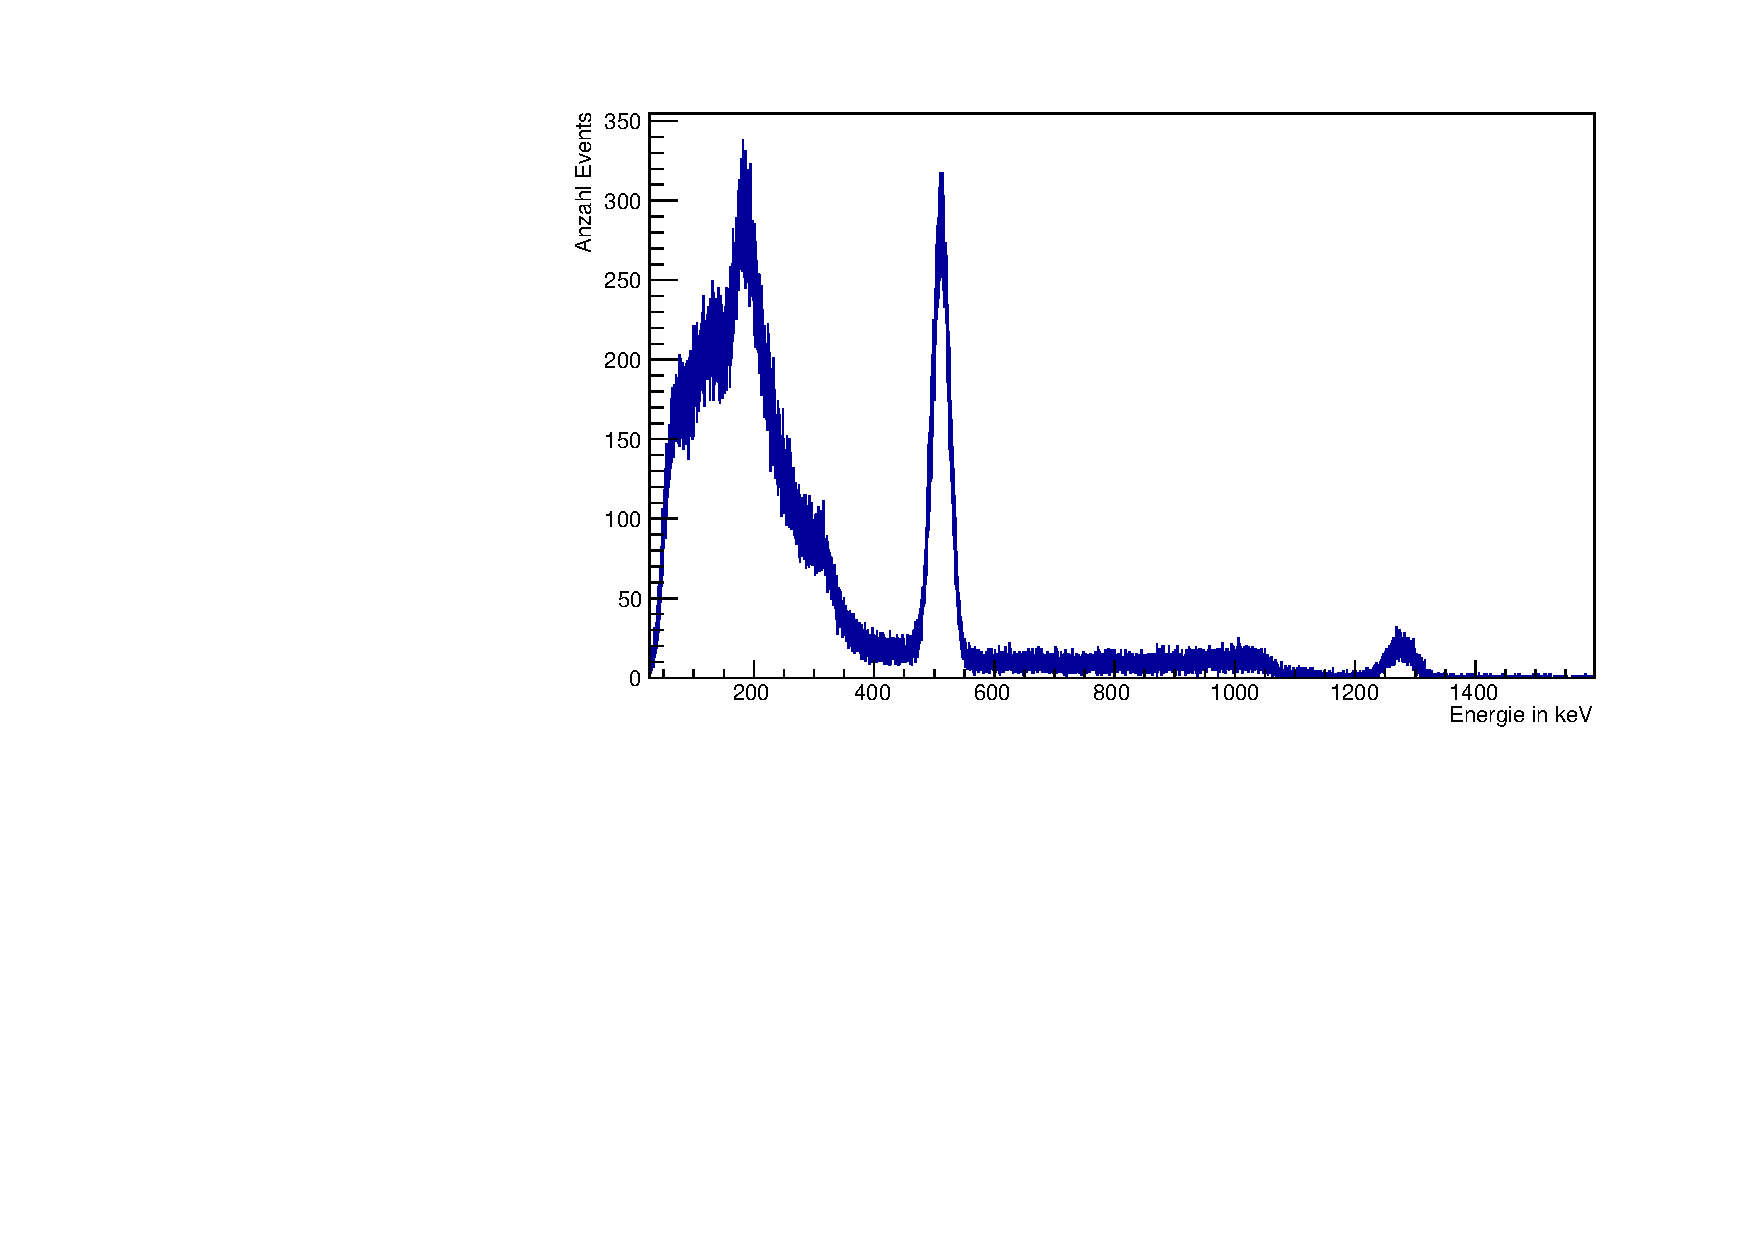
\includegraphics[width=\textwidth]{Messung11.pdf}
		\caption{Spektrum der 1. Messung}
		\label{l1}
	\end{center}
\end{figure}
Um die Auflösung der Detektoren zu bestimmen werden die Peaks über eine Gaußkurve angenähert. Die Auflösung wird als die Halbwertsbreite definiert, die bei einer Normalverteilung bei 1,35$\sigma$ liegt. Bei der ersten Messung ergibt sich bei einem Fit von 470 keV bis 550 keV ein $\sigma$ von 15,77 keV. Ein Fit von 1200 keV bis 1350 keV liefert ein Sigma von 22,34 keV. Abbildung \ref{l2} zeigt den Fit des ersten Peaks. Damit ergibt sich eine Auflösung von 21,29keV bei 511 keV sowie von 30,15 keV bei 1275keV.
\begin{figure}[htbp]
	\begin{center}
		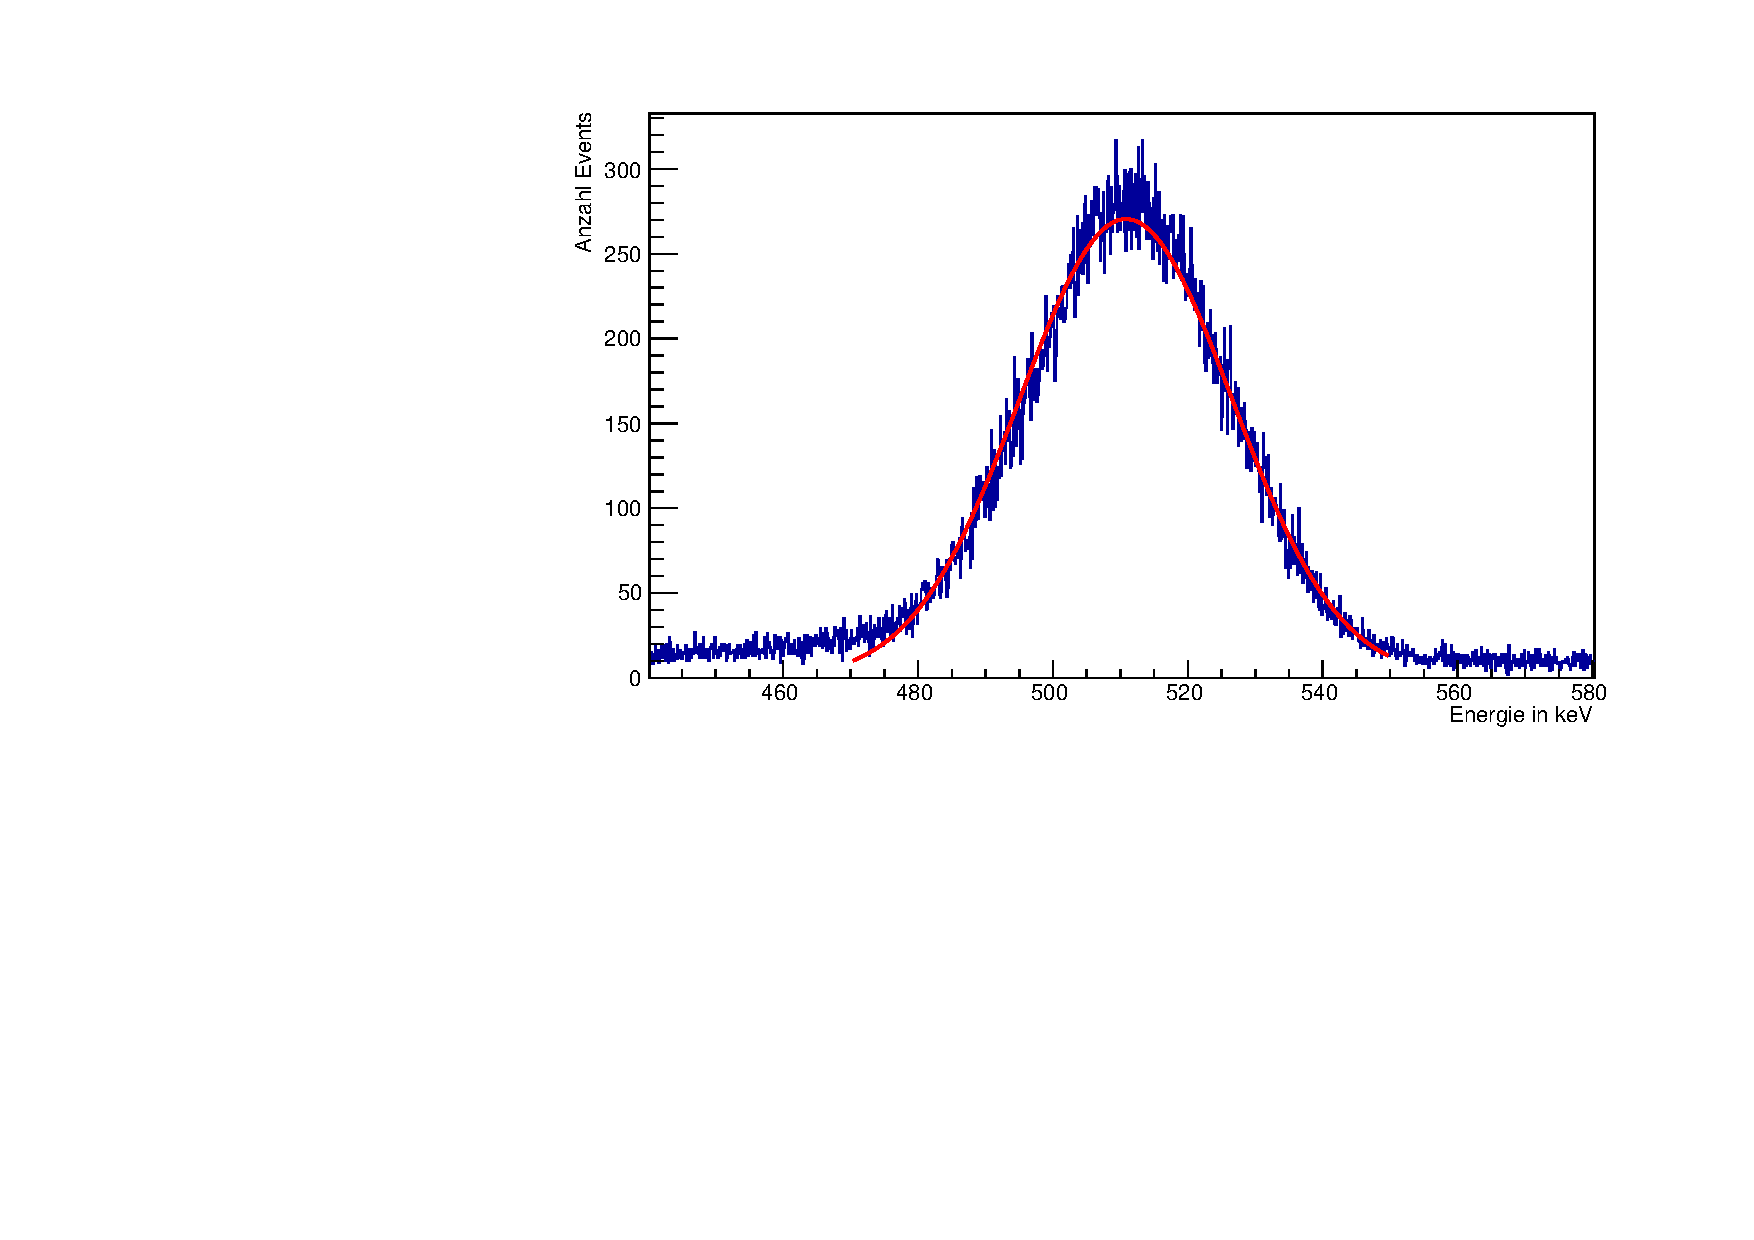
\includegraphics[width=\textwidth]{Fit1.pdf}
		\caption{Gaußscher Fit des 511 keV Peaks der ersten Messung}
		\label{l2}
	\end{center}
\end{figure}
\\\\
Die Effizienz setzt sich zusammen aus der geometrischen Effizienz und der Detektoreffizienz. Die geometrische Effizienz ist der Anteil des gesamten Raumwinkels den der Detektor abdeckt und wird über folgenden Ausdruck genähert:
\begin{equation}
\eta_{geometrisch}={A\over 4 \pi d^2}
\end{equation}
Die Photopeakeffizienz ergibt sich damit als
\begin{equation}
\eta_{Photopeak}={N_{peak}\over N_0*\eta_{geometrisch}}
\end{equation}
Wobei $N_0$ die Anzahl der emitierten Photonen ist, die sich aus der Aktivität ergibt. Der kleine Detektor besteht aus 2 Kristallen der Frontfläche 29*13$mm^2$, hat also eine Fläche A=754$mm^2$. Bei der ersten Messung betrug der Abstand zur Detektorbox 3cm, der Gesamtabstand also 4cm. Damit ergibt sich eine geometrische Effizienz von 3,75\%. Zusammen mit der Aktivität von 164,11kBq sowie der Messzeit von 7 Minuten ergibt sich eine Photopeakffizienz von
\begin{equation}
\eta_{Photopeak}={87710\over 7*60*164110*0,0375}=3,4\%
\end{equation}
Analog ergibt sich für die zweite Messung eine Auflösung von 20,91keV bzw 31,293keV und eine Effizienz von $\eta_{geometrisch}=2,4\%$ und $\eta_{Photopeak}=2,9\%$
%\bibliographystyle{alpha}
%\bibliographystyle{apalike}
%\bibliographystyle{plain}
%\bibliography{Literaturverzeichniss-Brue}
%\appendix
%\listoffigures
%\listoftables
%
\end{document} 